\subsection{Lift and bucket for debris}

\subsubsection{Lift}
The lift consists of two beams. One beam is stationar and it is fixed vertically on the back part of the robot. The second beam turns by DC motor that mounted at the top of stationar beam. The length of beams must allow to score debris to high goal from the middle zone and to middle goal from low zone.	\newline
For estimating optimal length of beams it was made drawing in GeoGebra.
\begin{figure}[H]
	\begin{minipage}[h]{1\linewidth}
		\center{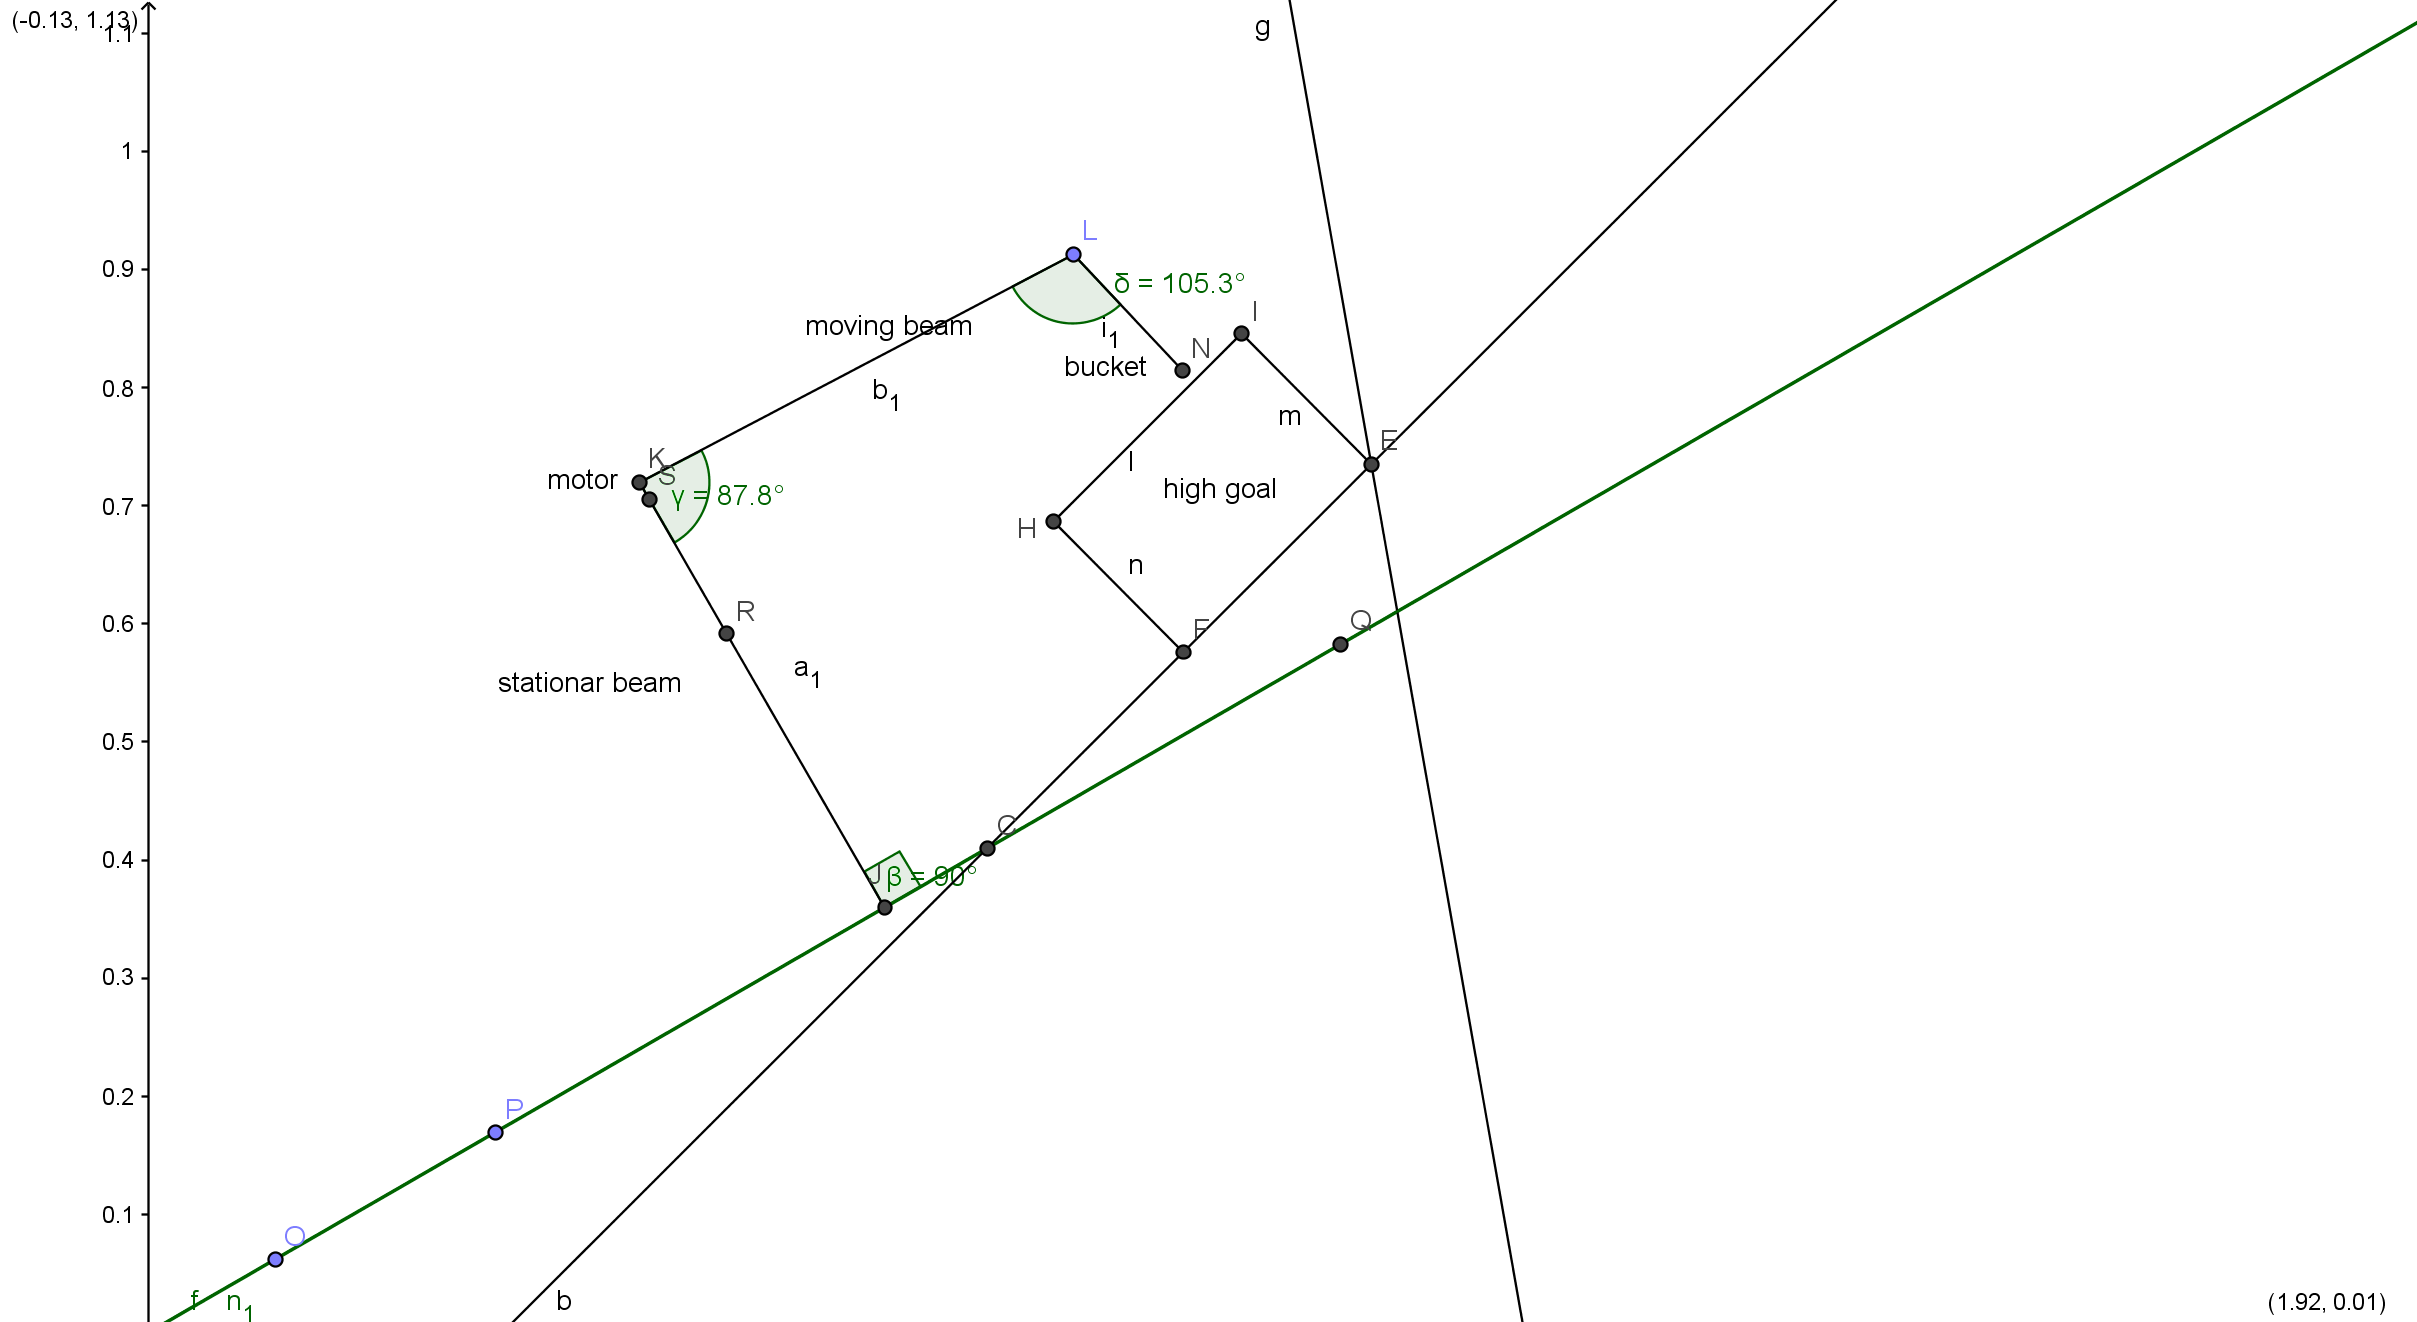
\includegraphics[scale=0.7]{days_L/Lift+bucket/images/02}}
		\caption{Drawing of the lift}
	\end{minipage}
\end{figure}

\subsubsection{Bucket} 
The bucket's size allow to fit 3 cubes and 2 balls.	\newline
For estimating optimal size and form it was made drawing in GeoGebra.
\begin{figure}[H]
	\begin{minipage}[h]{1\linewidth}
		\center{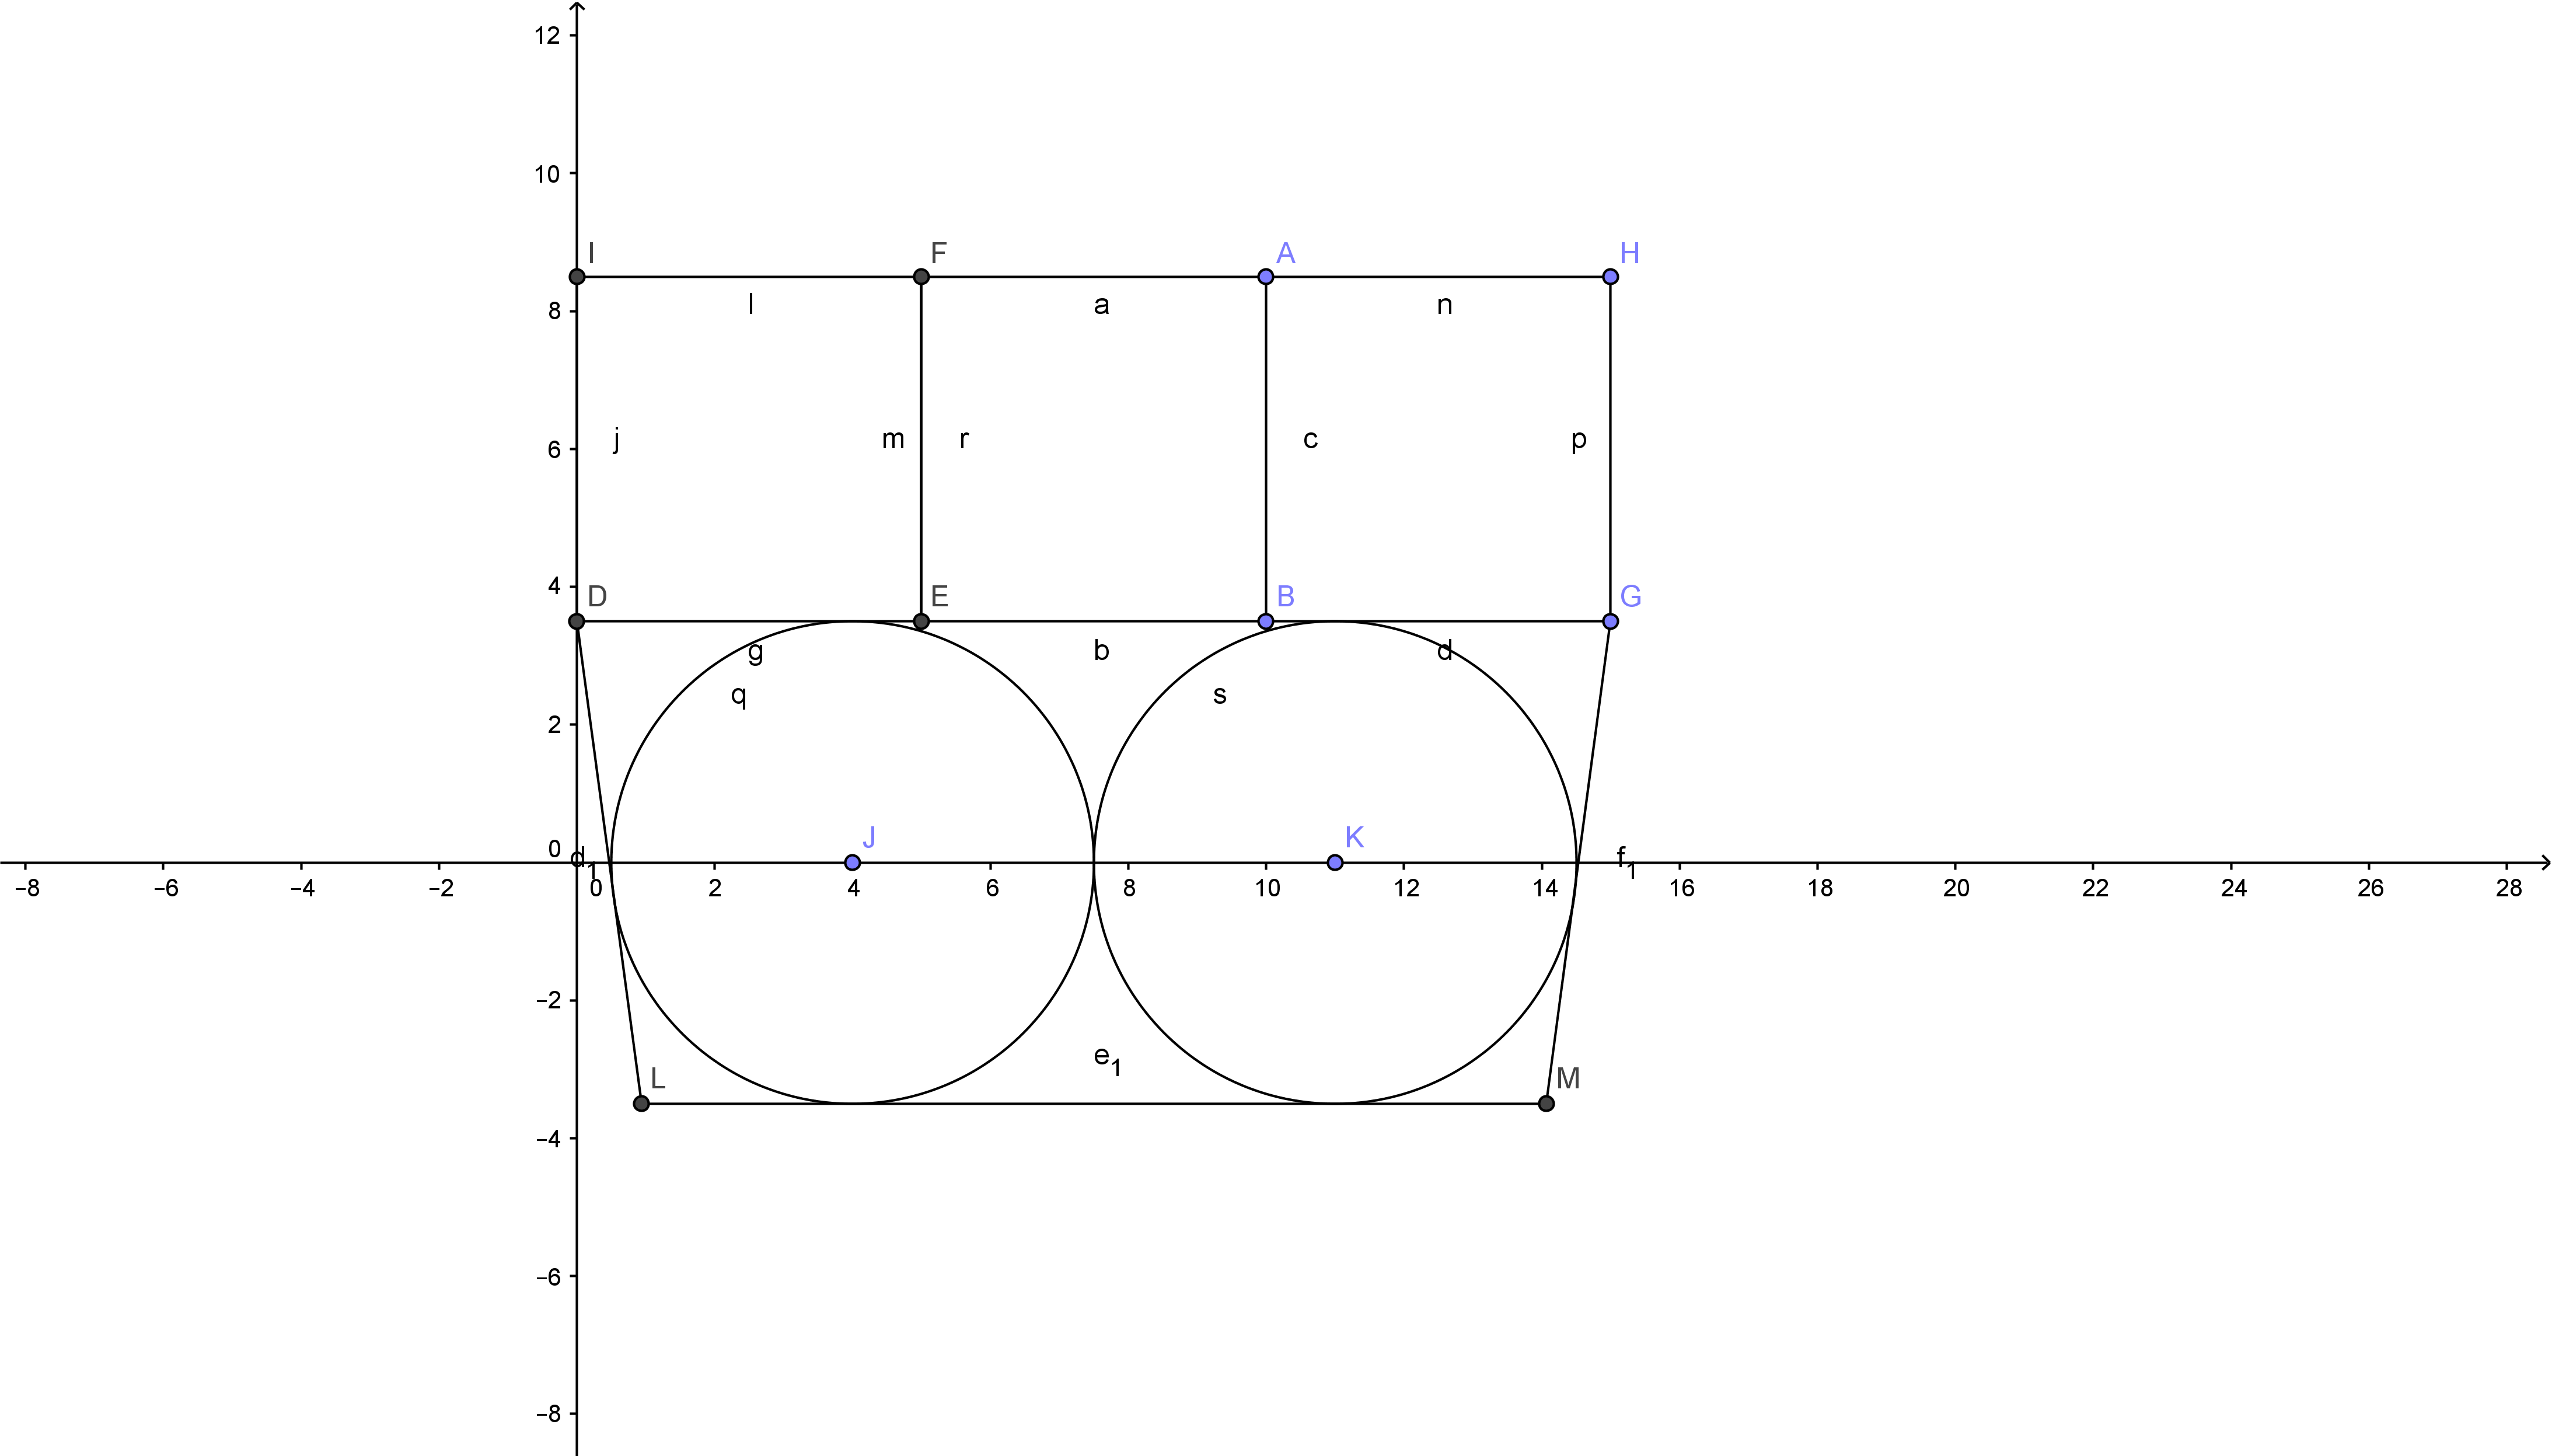
\includegraphics[scale=0.5]{days_L/Lift+bucket/images/01}}
		\caption{Drawing of the bucket}
	\end{minipage}
\end{figure}  

The bucket mounts to beam that turns by the servo which fixed on the lift. It need because else we have to make detail that fix bucket to the elevator on the defined angle. It require high accuracy. So it will be difficult to make this detail. In addition the mount with servo extend operational window of the lift.

  	
   	
\fillpage
